% !TeX root = ../main.tex
% Add the above to each chapter to make compiling the PDF easier in some editors.

% TODO: I have to rework the conclusion yet, to make it different from the paper
\chapter{Conclusion}\label{chapter:conclusion}

In this thesis, the performance of different label-efficient learning strategies, is investigated for biomedical image classification. First, it is shown that for classifying white blood cells into 10 different classes, active learning can boost macro recall. Second, it is shown that using ImageNet and SimCLR pre-training can increase the performance further. However, their contribution is dataset dependent: While for white blood cell and skin lesion dataset, ImageNet weight led to better performance, SimCLR performed better for classifying cell cycles (Figure 3). This might be due to the nature of images: Cell cycle data is captured by fluorescent imaging which follows a very different color distribution than other technologies such as dermoscopy cameras, which are closer to natural images. Therefore, ImageNet pre-training might not be the preferred way for such data.
It is also shown that by incorporating unlabeled data in the training process in a semi-supervised manner, one can improve the performance of the classification noticeably. Finally, by doing a grid-search over all the possible algorithms and strategies (Table 1), it is found that the combination of ImageNet or SimCLR pre-training, FixMatch semi-supervised learning and augmentation-based sampling can improve existing methods for every dataset. The reason for this is probably the fact that while training FixMatch, the network faces many different augmentations for each image and learns to make a robust prediction. Augmentation-based sampling relies on the same idea for finding those images where predictions were not robust enough. 

As a result of this study, an label-efficient strategy is proposed for biomedical imaging active learning tasks where unlabeled data is abundant (Figure 4). The strategy is split into two parts including pre-training and active learning. First, it is suggested to pre-train the network using SimCLR. Then compare FixMatch initialized with ImageNet weights to SimCLR pre-training. By comparing the results, select the best pre-training method. Eventually for the active learning part, it is recommended to train FixMatch along with the best pre-training method and augmentation-based sampling to obtain optimal results.

Although this thesis shows potential for improvement of label-efficient learning for three biomedical image classification datasets, the methodology should be tested on more datasets to gain insights into correlations between dataset characteristics and the performance of the applied methods. Due to the computational costs a fixed architecture is used with a fixed set of parameters. As the next step, different architectures will be tried with different parameters and the results will be evaluated accordingly. Also, a variety of active learning, semi-supervised and self-supervised learning methods should be added to the work to find the optimal strategy. Finally, to make the findings relevant to the biomedical deep learning field, implementations of the combined methods that allow for quick and easy application need to be provided in an open source implementation.

% Also remake this figure
\begin{figure}[htbp]
\centering
\captionsetup{format=plain}
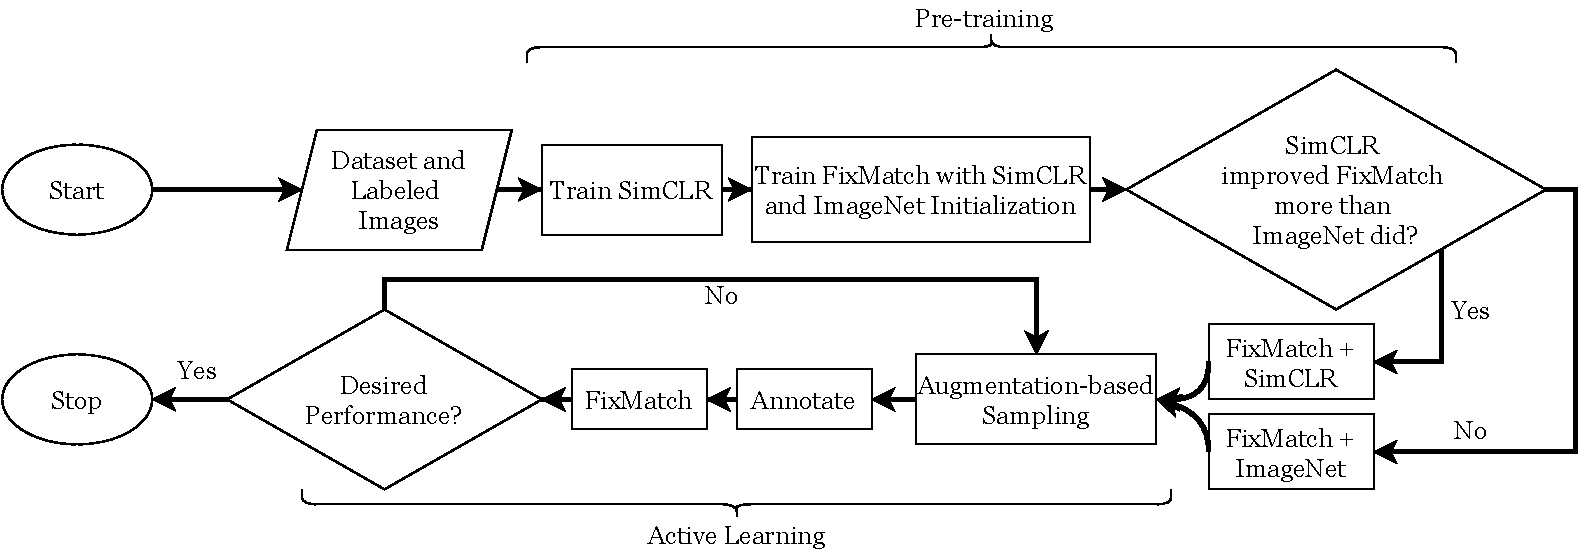
\includegraphics[width=\textwidth]{figures/fig_conclusion.pdf}
\caption[Recommended Strategy]{Recommended strategy for label-efficient classification of biomedical image data involves SimCLR or ImageNet pre-training, FixMatch as the semi-supervised algorithm for training and augmentation-based sampling during active learning until the desired performance is reached.}
\label{fig:fig_conclusion}
\end{figure}